% Compile with: pdflatex --shell-escape waveguide_tikz.tex
\documentclass[tikz,border=10pt]{standalone}
\usepackage{tikz}
\usepackage{amsmath}
\begin{document}

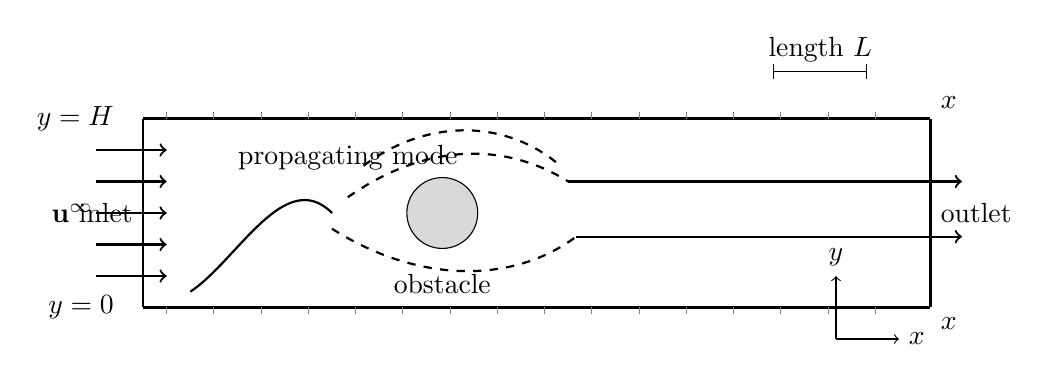
\begin{tikzpicture}[scale=1, every node/.style={scale=1}]
  % Parameters
  \def\L{10} % length of waveguide
  \def\H{2.4} % height of waveguide
  \def\obsx{3.8} % obstacle x
  \def\obsy{1.2} % obstacle y (center)
  \def\r{0.45} % obstacle radius

  % waveguide walls
  \draw[thick] (0,0) -- (\L,0) node[below right] { $x$ };
  \draw[thick] (0,\H) -- (\L,\H) node[above right] { $x$ };

  % side boundaries (left and right)
  \draw[thick] (0,0) -- (0,\H) node[midway,left] { inlet };
  \draw[thick] (\L,0) -- (\L,\H) node[midway,right] { outlet };

  % labels for walls
  \node at (-0.25,0) [left] { $y=0$ };
  \node at (-0.25,\H) [left] { $y=H$ };

  % obstacle (circle)
  \filldraw[fill=gray!30, draw=black] (\obsx,\obsy) circle (\r) ;
  \node at (\obsx,\obsy-0.9) { obstacle };

  % Mesh-like boundary elements on top/bottom (optional)
  % draw some short ticks on walls to suggest boundary
  \foreach \x in {0.3,0.9,1.5,2.1,2.7,3.3,3.9,4.5,5.1,5.7,6.3,6.9,7.5,8.1,8.7,9.3}
    {\draw[gray] (\x,0) -- (\x, -0.08); \draw[gray] (\x,\H) -- (\x,\H+0.08);} 

  % incoming uniform flow arrows (left to right)
  \foreach \y in {0.4,0.8,1.2,1.6,2.0}
    {\draw[->,thick] (-0.6,\y) -- (0.3,\y);}
  \node at (-0.9,1.2) { $\mathbf{u}^{\infty}$ };

  % scattered field sketch: curved streamlines around obstacle (simple)
  \draw[thick, dashed] (\obsx-1.2,\obsy+0.2) .. controls (\obsx-0.2,\obsy+0.9) and (\obsx+0.8,\obsy+0.9) .. (\obsx+1.6,\obsy+0.4);
  \draw[thick, dashed] (\obsx-1.4,\obsy-0.2) .. controls (\obsx-0.3,\obsy-0.9) and (\obsx+0.9,\obsy-0.9) .. (\obsx+1.7,\obsy-0.3);
  \draw[thick, dashed] (\obsx-1.0,\obsy+0.6) .. controls (\obsx-0.2,\obsy+1.2) and (\obsx+0.8,\obsy+1.2) .. (\obsx+1.5,\obsy+0.6);

  % scattered wave arrows leaving right
  \draw[->, thick] (\obsx+1.6,\obsy+0.4) -- (\L+0.4,\obsy+0.4);
  \draw[->, thick] (\obsx+1.7,\obsy-0.3) -- (\L+0.4,\obsy-0.3);

  % coordinate system for reference near bottom right
  \draw[->] (\L-1.2,-0.4) -- (\L-0.4,-0.4) node[right] {$x$};
  \draw[->] (\L-1.2,-0.4) -- (\L-1.2,0.4) node[above] {$y$};

  % scale bar
  \draw[|-|] (\L-2,\H+0.6) -- (\L-0.8,\H+0.6) node[midway,above] { length $L$ };

  % optional annotation for mode shape (simple sine)
  \draw[thick] (0.6,0.2) .. controls (1.2,0.6) and (1.8,1.8) .. (2.4,1.2);
  \node at (2.6,1.9) { propagating mode };

\end{tikzpicture}

\end{document}
